\documentclass[tikz,border=2pt]{standalone}
\usepackage{amsmath,amssymb}
\usepackage{pgfplots}
\pgfplotsset{compat=1.18}
\usetikzlibrary{arrows.meta}
\begin{document}
% Base-stock policy, Lighthouse case: S = 9, lead time 2, I = S - X has pmf P(I = 9 - k) = P(X = k),
% k = 0..10; the only negative value I = -1 (backlog) has probability 1/36; E[I] = 9 - 4.55 = 4.45.
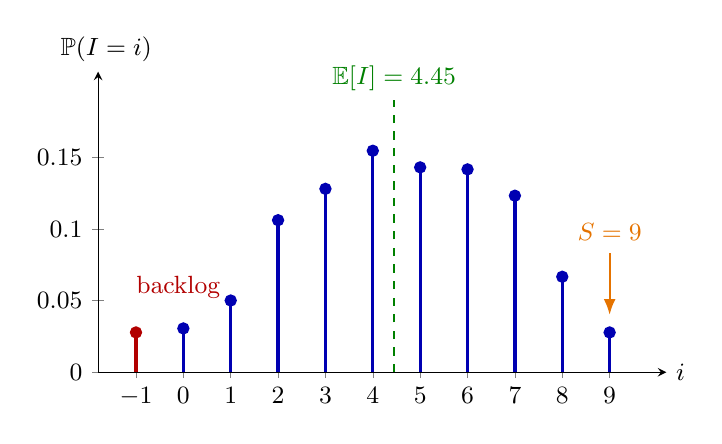
\begin{tikzpicture}[font=\small, >={Latex[length=2mm]}]
  \begin{axis}[axis lines=left, xmin=-1.8, xmax=10.2, ymin=0, ymax=0.21,
    xtick={-1,0,...,9}, ytick={0,0.05,0.1,0.15}, yticklabels={$0$,$0.05$,$0.1$,$0.15$},
    xlabel={$i$}, ylabel={$\mathbb{P}(I=i)$},
    xlabel style={at={(axis description cs:1,0)}, anchor=west},
    ylabel style={rotate=-90, at={(axis description cs:0,1)}, anchor=south west, xshift=-6mm},
    width=8.8cm, height=5.4cm, clip=false]
    \addplot[ycomb, blue!70!black, very thick, mark=*, mark size=1.6pt]
      coordinates {(9,0.0278) (8,0.0667) (7,0.1233) (6,0.1417) (5,0.1431) (4,0.1547)
                   (3,0.1281) (2,0.1062) (1,0.0501) (0,0.0306)};
    \addplot[ycomb, red!70!black, very thick, mark=*, mark size=1.6pt] coordinates {(-1,0.0278)};
    \node[red!70!black, anchor=south west] at (axis cs:-1.2,0.045) {backlog};
    \node[orange!90!black, anchor=south] at (axis cs:9,0.085) {$S=9$};
    \draw[orange!90!black, thick, ->] (axis cs:9,0.083) -- (axis cs:9,0.04);
    \draw[green!50!black, thick, dashed] (axis cs:4.45,0) -- (axis cs:4.45,0.19);
    \node[green!50!black, anchor=south] at (axis cs:4.45,0.19) {$\mathbb{E}[I]=4.45$};
  \end{axis}
\end{tikzpicture}
\end{document}
